% This text is proprietary.
% It's a part of presentation made by myself.
% It may not used commercial.
% The noncommercial use such as private and study is free
% May 2007
% Author: Sascha Frank 
% University Freiburg 
% www.informatik.uni-freiburg.de/~frank/
%
% 
\documentclass{beamer}
\setbeamertemplate{navigation symbols}{}

\usepackage{beamerthemeshadow}
\begin{document}
\title{PPI Networks and Gene Expression}  
\author{Adrin Jalali}
\date{\today} 

\begin{frame}
\titlepage
\end{frame}

%\begin{frame}\frametitle{Table of contents}\tableofcontents
%\end{frame} 


\section{Formulation} 
\begin{frame}
\frametitle{SVM} 

\begin{block}{SVM problem}
\begin{center}
  $\min_{\mathbf{w}, w_0}\left\{\frac{1}{2}\|\mathbf{w}\|^2 + \frac{1}{2}\beta\sum_{(j,k)\in E}(w_j-w_k)^2\right\}$
\end{center}
subject to
\begin{center}
  $\forall i \in \{1,\cdots,n\} : (\mathbf{w}x_i+w_0)y_i\geq 1$
\end{center}
\end{block}
\end{frame}

\begin{frame}
\frametitle{Dual}
\begin{block}{Dual problem}
  \begin{center}
    \begin{align*}
    &\max_\alpha\left\{\sum_{i=1}^n\alpha_i-\frac{1}{2}\sum_{i=1}^n\sum_{j=1}^n\alpha_i\alpha_j y_i y_j (x_i^TL)(L^Tx_j)\right\}\\
      &LL^T=(I+\beta B)^{-1}\\
        \text{s.t.: }&\\
        &\forall i \in \{1,\cdots,n\}: \sum_{i=1}^n\alpha_iy_i=0\\
        &\forall i \in \{1,\cdots,n\}: \alpha_i \geq 0
    \end{align*}
  \end{center}
\end{block}
\end{frame}

\section{Results}
\begin{frame}
\frametitle{Synthesize data}
\begin{enumerate}
\item A random graph
\item Signal nodes: \[ f(n) = \left\{ 
  \begin{array}{l l}
    N(-\mu, 1) & \quad \text{if $n$ is in class $1$}\\
    N(\mu, 1) & \quad \text{if $n$ is in class $2$}
  \end{array} \right.\]
\item Random nodes: \[f(n) = N(0, 1) \]
\item Pathway: 2, 3, or 4 connected signal nodes.
\end{enumerate}
\end{frame}

\begin{frame}[plain]
\frametitle{Synthesized data}
\begin{figure}
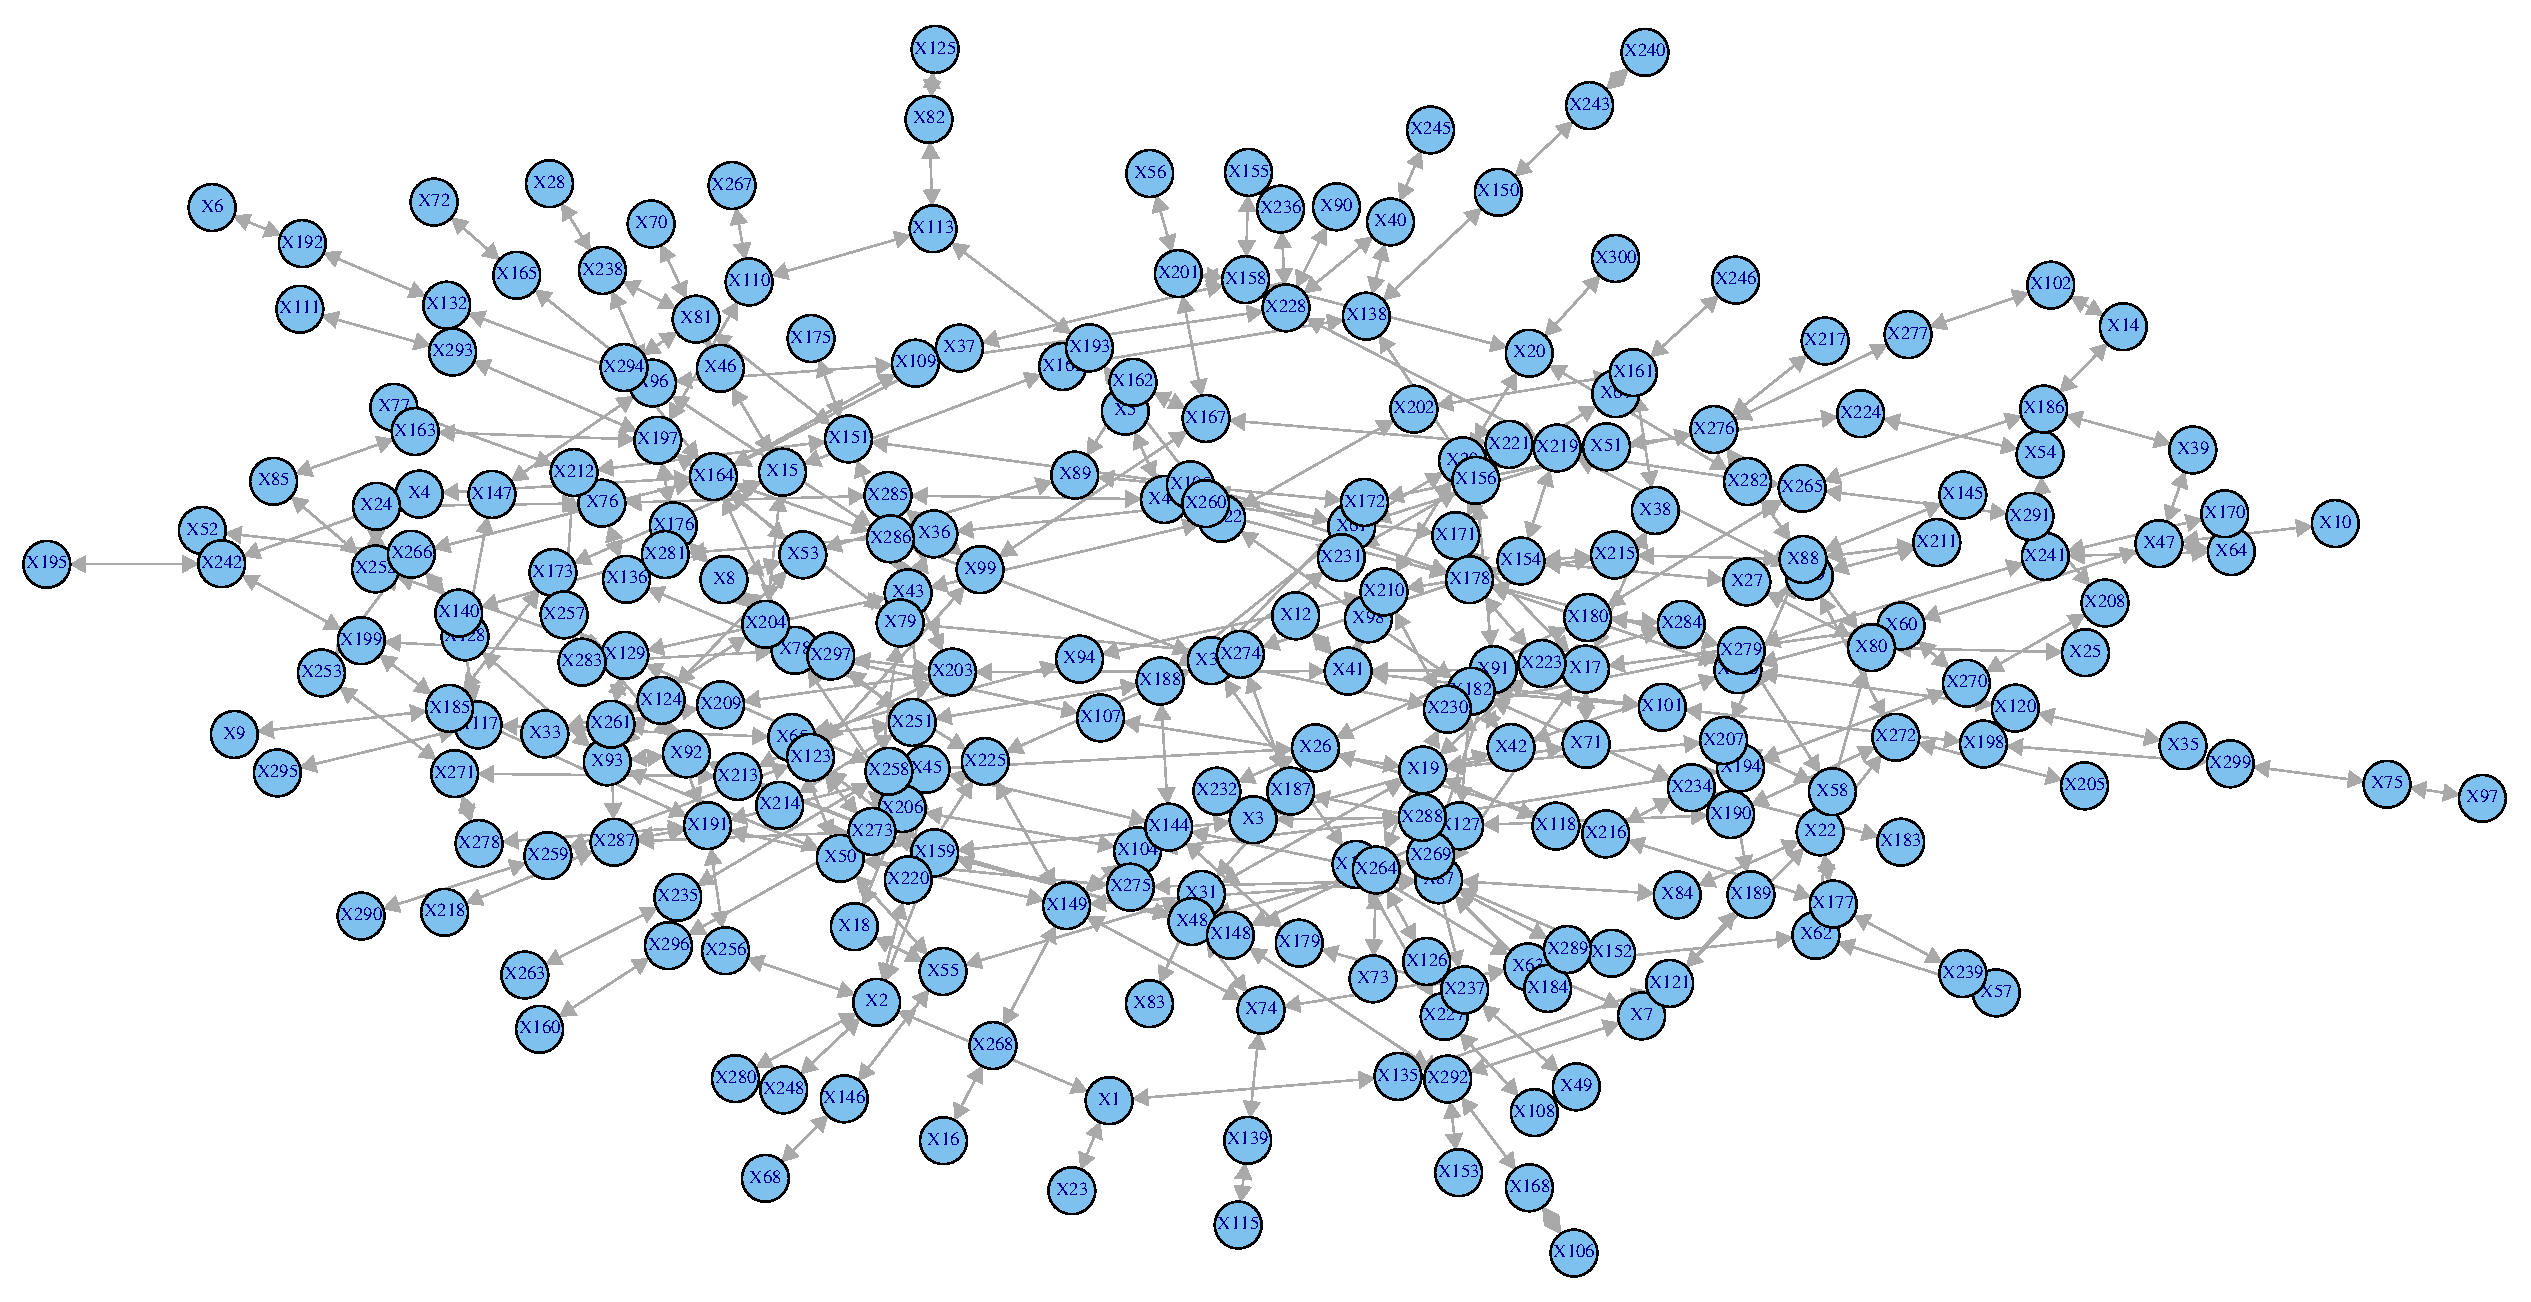
\includegraphics[scale=0.25]{synthesized-graph} 
\end{figure}
\end{frame}

\begin{frame}[plain]
\frametitle{Synthesized data easy scenario}
\begin{figure}
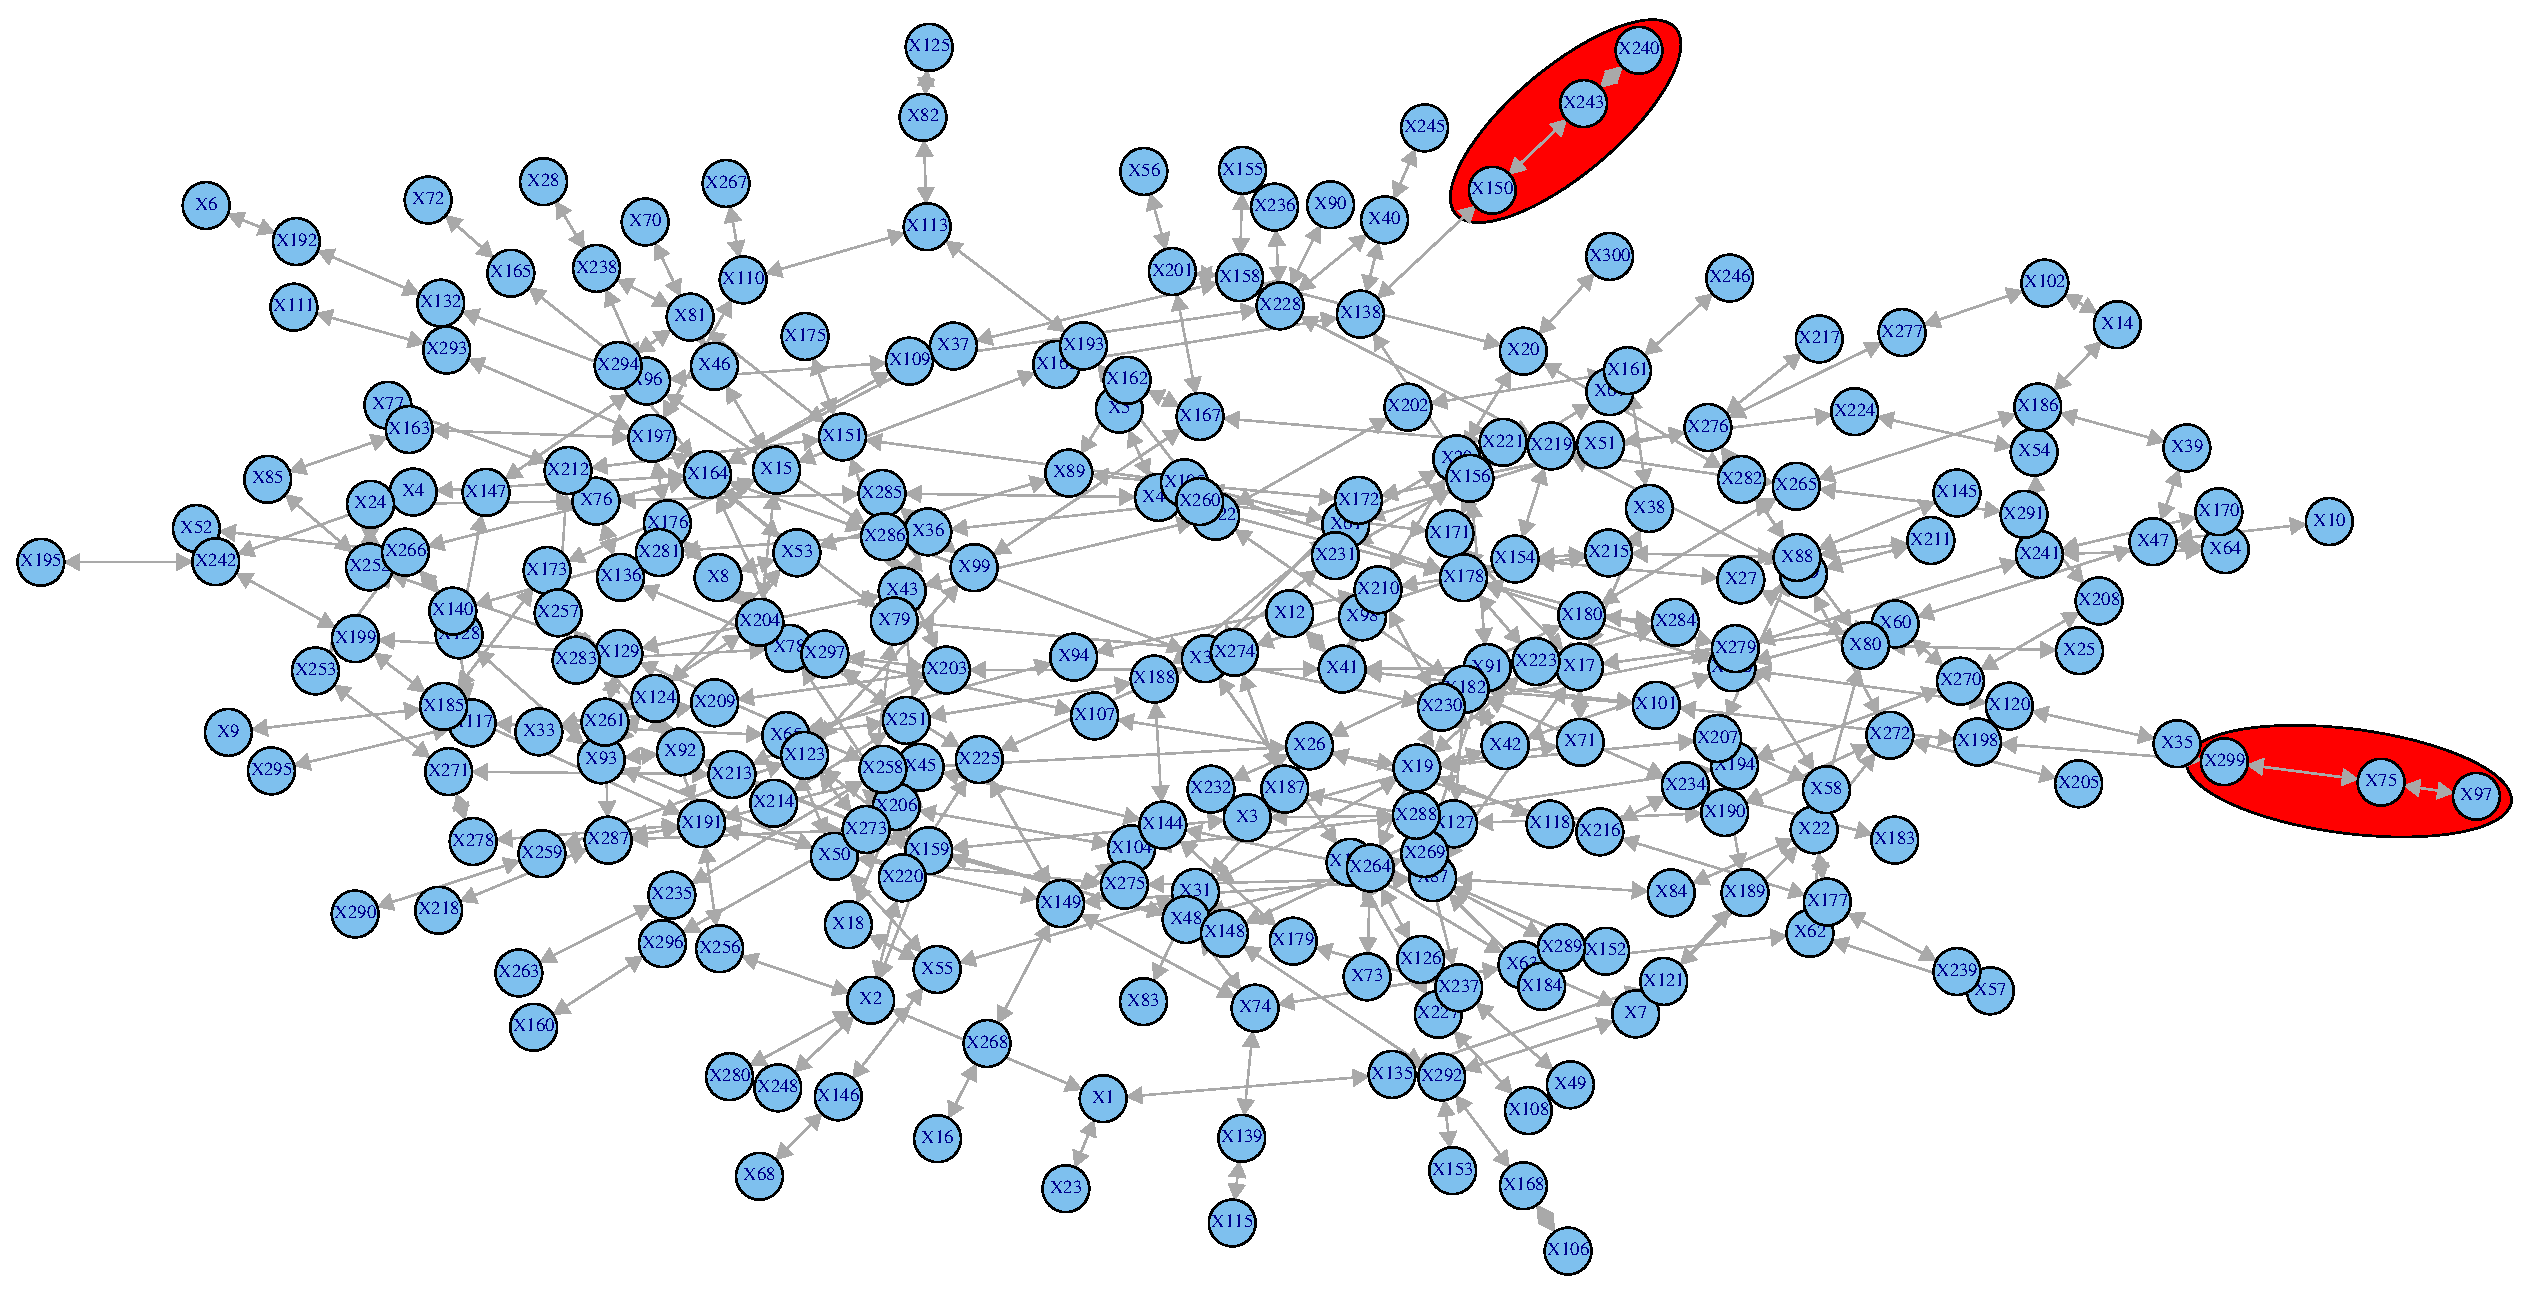
\includegraphics[scale=0.25]{synthesized-graph-easy} 
\end{figure}
\end{frame}

\begin{frame}[plain]
\frametitle{Synthesized data hard scenario}
\begin{figure}
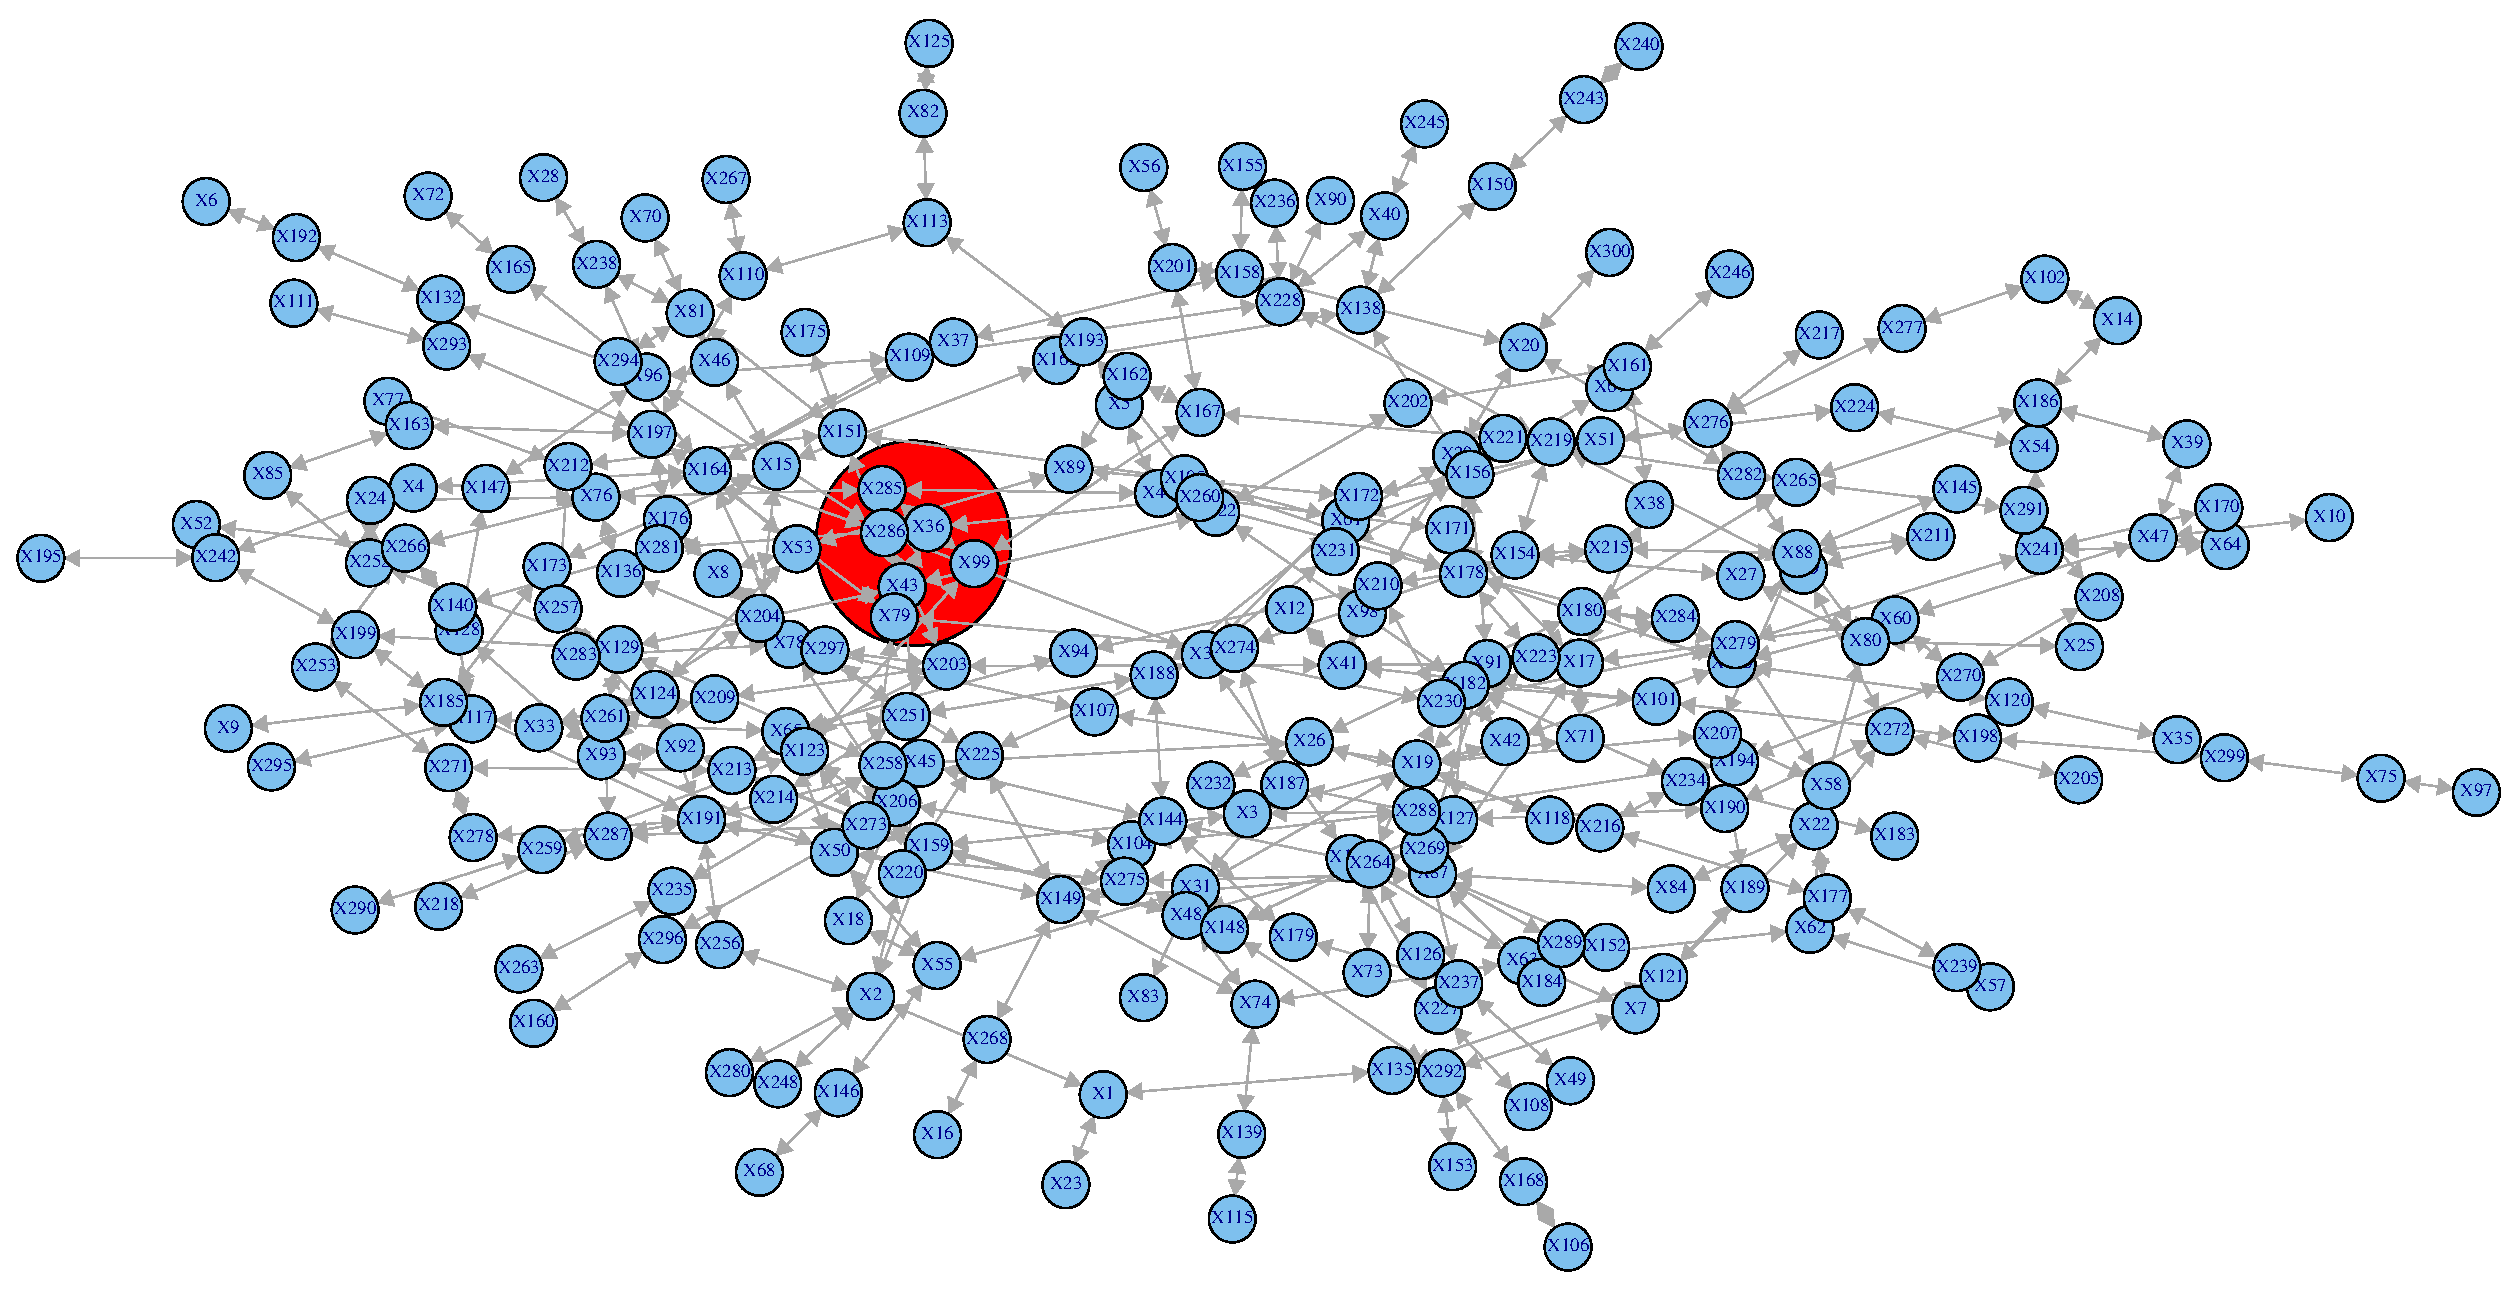
\includegraphics[scale=0.25]{synthesized-graph-hard}
\end{figure}
\end{frame}

\begin{frame}
\frametitle{Results}
\begin{enumerate}
\item Extract pairs of genes with mutual absolute large $w$ 
\item Synthesized easy: all implanted pathways come on top of the list 
\item Synthesized hard: they are vanished \pause
\item Van't veer: 
  \begin{enumerate}
    \item Slightly better performance, although not necessarily as reported.
    \item You find even better genes in w/o network scenario.
    \item Well known genes are of very high degree in the network.
  \end{enumerate}
\end{enumerate}
\end{frame}

\section{Idea}
\begin{frame}
\frametitle{Idea}
\begin{enumerate}
\item Estimate density distribution of each gene for class A. \pause
\item For each sample:
  \begin{enumerate}
  \item Extract abnormal genes according to above estimated distributions.
  \item Extract the part of PPI network induced by extracted genes (almost)
  \end{enumerate}\pause
\item Use a graph kernel for labeled graphs to classify extracted graphs. \pause
\item Extract common sub-graphs from individual graphs that seem to be helping the classification.
\end{enumerate}
\end{frame}

\begin{frame}[plain]
\frametitle{Finished!}
  \begin{center}
    \Huge{Thank You!}
  \end{center}
\end{frame}

\end{document}
